%%%%%%%%%%%%%%%%%%%%%%%%%%%%%%%%%%%%%%%%%%%%%%%%%%%%%%%
% % Lines starting with % are comments, which are ignored.
% % This is a handy way of indicating the date and version of
% % your document, to wit:
% %
% % LaTeX sample file
% % Modified March, 2002
% %
%%%%%%%%%%%%%%%%%%%%%%%%%%%%%%%%%%%%%%%%%%%%%%%%%%%%%%%
\DocumentMetadata{
  % PDF standards: ONE key whose value is a comma-separated list --
  % UA-2 (accessibility) plus A-4f (archival; the archival companion of
  % UA-2). Do NOT use separate pdfstandard=... keys: with ordinary
  % key-value parsing only the last one takes effect.
  pdfstandard={UA-2,A-4f},
  lang=en-US,
  tagging=on,
  tagging-setup={
    math/setup=mathml-SE
  }
}

\documentclass[12pt]{exam}
% worksheet-macros.tex -- shared package setup for worksheet-template.tex.
%
% NOTE ON PATHS: every template in this repository is stored one level up
% from where it is compiled (see README.md). All relative \input paths
% below are resolved against the folder the document is compiled in,
% which sits one directory above this file.

% --- Math ------------------------------------------------------------
% amsmath: equation environments and numbering
% amsfonts: \mathbb etc.  |  mathrsfs: \mathfrak  |  stmaryrd: extra symbols
\usepackage{amsmath}
\usepackage{amsfonts}
\usepackage{mathrsfs}
\usepackage{stmaryrd}

% --- Layout and glyphs ------------------------------------------------
% float: [H] float placement (stop floats where you put them)
% fontspec: Unicode/OpenType fonts (compile with XeLaTeX or LuaLaTeX)
% emoji: emoji glyphs in the text
\usepackage{float}
\usepackage{fontspec}
\usepackage{emoji}

% --- Typography --------------------------------------------------------
% Atkinson Hyperlegible as the document-wide sans serif (sfdefault):
% a high-legibility face that is easier to read for students with
% dyslexia or low vision.
\usepackage[sfdefault]{atkinson}

% --- Colors -------------------------------------------------------------
% dvipsnames: extended named color palette (the Accessible* colors in
%   lecture-macros.tex are built on it);
% table: \rowcolors / \cellcolor for shading worksheet tables.
% NOTE: xcolor may only be loaded ONCE per document -- a second
% \usepackage{xcolor} with different options is a fatal "Option clash"
% error, so ALL of its options are listed here.
\usepackage[dvipsnames,table]{xcolor}

% --- Multimedia ---------------------------------------------------------
% animate: embeds audio/video (and legacy Flash) media in the worksheet.
\usepackage{animate}

% --- Bibliography --------------------------------------------------------
% biblatex (biber backend): citations and a reference list for worksheets.
\usepackage[
  backend=biber,
  style=alphabetic,
  url=true,
  doi=true,
  isbn=true,
  backref=true
]{biblatex}

% --- Links ---------------------------------------------------------------
% hyperref makes every \ref/citation/URL clickable in the PDF.
% Link colors must satisfy WCAG 1.4.3 (>= 4.5:1 contrast on white):
%   blue = 8.6:1, green!40!black = 7.2:1.
% (The old cyan/magenta values measured 1.25:1 / 3.1:1 and failed.)
\usepackage{hyperref}
\hypersetup{
  colorlinks=true,
  linkcolor=blue,
  filecolor=blue,
  urlcolor=green!40!black,
}

% --- Shared course macros ------------------------------------------------
% Root macros.tex: math shorthands used across all course documents
% (\RR, \NN, \ZZ, \QQ, \grad, \curl, \tr, \der, \pder, ...).
\newcommand{\RR}{\mathbb{R}}
\newcommand{\NN}{\mathbb{N}}
\newcommand{\ZZ}{\mathbb{Z}}
\newcommand{\QQ}{\mathbb{Q}}
\newcommand{\vv}{\vec{v}}
\newcommand{\ww}{\vec{w}}
\newcommand{\xx}{\vec{x}}
\newcommand{\yy}{\vec{y}}
\newcommand{\zz}{\vec{z}}
\newcommand{\uu}{\vec{u}}
\newcommand{\basis}[1]{\vec{e_{#1}}}
\newcommand{\id}{\mathrm{id}}
\newcommand{\CC}{\mathbb{C}}
\renewcommand{\div}{\operatorname{div}}
\newcommand{\grad}{\operatorname{grad}}
\newcommand{\curl}{\operatorname{curl}}
\newcommand{\tr}{\operatorname{tr}}
\newcommand{\der}[2]{\dfrac{d #1}{d #2}}
\newcommand{\pder}[3][]{\dfrac{\partial^{#1} #2}{\partial #3}}


\usepackage{tikz}
\usepackage{multicol}
% % Title and author(s)
%%%%%%%%%%%%%%%%%%%%%%%%%%%%%%%%%%%%%%%%%%%%%%%%%%%%%%%
\title{Worksheet 3: Limits and Continuous Functions}
\author{MATH 2263}
\date{09/15/2026}
%%%%%%%%%%%%%%%%%%%%%%%%%%%%%%%%%%%%%%%%%%%%%%%%%%%%%%%
% %
% % The next command allows your in import encapsulated
% % postscript files, .epsf or .eps files, which
% % contain vector graphic image data.
% %
%%%%%%%%%%%%%%%%%%%%%%%%%%%%%%%%%%%%%%%%%%%%%%%%%%%%%%%
% %   The first thanks indicates your affiliation
% %
% %  Just the name here.
% %
% % Your mailing address goes at the end.
% %
% % \thanks is also how you indicate grant support
% %
%%%%%%%%%%%%%%%%%%%%%%%%%%%%%%%%%%%%%%%%%%%%%%%%%%%%%%%

%%%%%%%%%%%%%%%%%%%%%%%%%%%%%%%%%%%%%%%%%%%%%%%%%%%%%%%
% $ The next command ensures the margins are 1 inch on
% % all sides.
% %
%%%%%%%%%%%%%%%%%%%%%%%%%%%%%%%%%%%%%%%%%%%%%%%%%%%%%%%
\begin{document}
\newpage
\maketitle

\section{Determining Continuity}
\subsection{Graphically}
For the following problems let $f(x)$ and $g(x)$ be functions whose graphs are given below.
The graph of $f(x)$ is the solid graph, the graph of $g(x)$ is the dashed graph.

\begin{figure}[H]
  \centering
  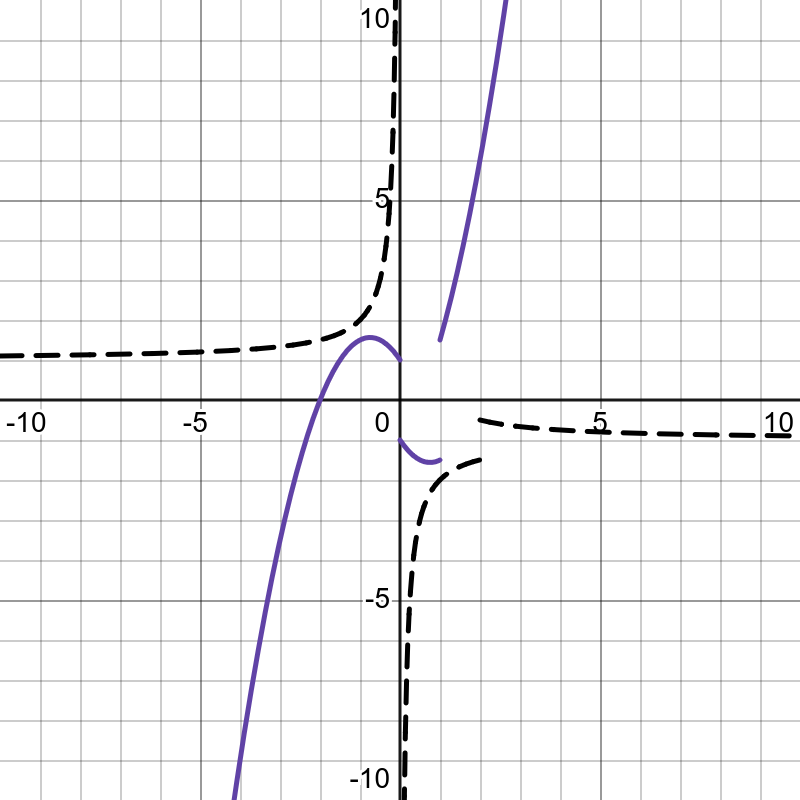
\includegraphics[width=0.3\textwidth]{Additivity Graph.png}
  \caption{Function Graphs}
\end{figure}

Determine if the following functions are continuous as the indicated points:
\begin{enumerate}
  \item Is $f(x)$ continuous at $-2$?
  \item Is $f(x)$ continuous at $-1$?
  \item Is $f(x)$ continuous at 0?
  \item Is $g(x)$ continuous at $0$?
  \item Is $g(x)^2 + f(x)$ continuous at $-2$?
  \item Is $f(x) + g(x)$ continuous at $2$?
  \item Is $f(x+1)^2 g(x-1)$ continuous at $0$?
\end{enumerate}

\newpage
\subsection{Algebraically}
\begin{enumerate}
  \item Is $f(x) = x^3 - 2x + 1$ continuous at $x = 0$? Why or why not?
  \vspace{\stretch{0.2}}

\item Is $g(x) = \dfrac{x^2 - 1}{x + 1}$ continuous at $x = -1$? Why or why not?
  \vspace{\stretch{0.2}}

\item Is $h(x) = \dfrac{\sin(x)}{x}$ a continuous function? Why or why not?
  \vspace{\stretch{0.2}}

\item Is the function $F(x) = \begin{cases} -x, & x < 0 \\ 0, & x = 0 \\ x, & x > 0 \end{cases}$ a continuous function? Why or why not?
  \vspace{\stretch{0.2}}

\item Is the function $G(x) = \begin{cases} x^3 - 3x^2 + 2x, & x \leq -2 \\ x + 2, & -2 < x < 2 \\ x^2 + \sin(x), & x \geq 2 \end{cases}$
  continuous on the interval $[-1, 1]$? Why or why not?
  \vspace{\stretch{0.2}}
\end{enumerate}
\newpage

\section{Computing Limits}
\subsection{Algebraically}
Compute the following limits algebraically, and explain your reasoning when/if you compute a limit by evaluation:

\begin{enumerate}
  \item $\displaystyle\lim_{x\to 1}\frac{x^2-1}{x-1}$

\vfill

\item $\displaystyle\lim_{x\to 0}\frac{(2+x)^3-8}{x}$

\vfill

\item $\displaystyle\lim_{x\to0}\frac{\sqrt{x+1}-1}{x}$

\vfill

\item $\displaystyle\lim_{x \rightarrow 1} \sin\left(\dfrac{x^2 - 2x + 1}{x - 1}\right)$

\end{enumerate}
\newpage
\subsection{Graphically}
Two functions, $f(x)$ and $g(x)$, are graphed below:

\begin{multicols}{2}

\begin{enumerate}

\item[]

\begin{tikzpicture}[scale=0.7]
 Grid
\draw[dotted] (-3.9,-3.9) grid (3.9,3.9); 
 Axes
\draw[<->] (-4,0) -- (4,0)node[anchor=north] {\footnotesize{$x$}};
\draw[->] (0,-4)--(0,4)node[anchor=east] {\footnotesize{$y$}};

\draw[very thick,-] [smooth,samples=100,domain=-2.3:3.33] plot({\x},{(1/3)*((\x)-1)^2});

\node at (1.5,-1.5) {$f(x)$};

\node[anchor=north] at (-1,0)  {$-1$};
\node[anchor=north] at (-2,0)  {$-2$};
\node[anchor=north] at (-3,0)  {$-3$};
\node[anchor=north] at (1,0)  {$1$};
\node[anchor=north] at (2,0)  {$2$};
\node[anchor=north] at (3,0)  {$3$};

\node[anchor=east] at (0,-3)  {$-3$};
\node[anchor=east] at (0,-2)  {$-2$};
\node[anchor=east] at (0,-1)  {$-1$};
\node[anchor=east] at (0,1)  {$1$};
\node[anchor=east] at (0,2)  {$2$};
\node[anchor=east] at (0,3)  {$3$};
\end{tikzpicture}

\columnbreak

\item[]

\begin{tikzpicture}[scale=0.7]
 Grid
\draw[dotted] (-3.9,-3.9) grid (3.9,3.9); 
 Axes
\draw[<->] (-4,0) -- (4,0)node[anchor=north] {\footnotesize{$x$}};
\draw[->] (0,-4)--(0,4)node[anchor=east] {\footnotesize{$y$}};

\draw[very thick,-] [smooth,samples=100,domain=-2:-0.05] plot({\x},{(\x)-2});

\node at (0,-2) {$\circ$};

\node at (0,1) {$\bullet$};

\node at (0,3) {$\circ$};

\node at (-1.5, 2.5) {$g(x)$};

\draw[very thick,-] [smooth,samples=100,domain=0.05:2.5] plot({\x},{3-(\x)^2});

\node[anchor=north] at (-1,0)  {$-1$};
\node[anchor=north] at (-2,0)  {$-2$};
\node[anchor=north] at (-3,0)  {$-3$};
\node[anchor=north] at (1,0)  {$1$};
\node[anchor=north] at (2,0)  {$2$};
\node[anchor=north] at (3,0)  {$3$};

\node[anchor=east] at (0,-3)  {$-3$};
\node[anchor=east] at (0,-2)  {$-2$};
\node[anchor=east] at (0,-1)  {$-1$};
\node[anchor=east] at (0,1)  {$1$};
\node[anchor=east] at (0,2)  {$2$};
\node[anchor=east] at (0,3)  {$3$};
\end{tikzpicture}

\end{enumerate}
\end{multicols}

(If necessary, you may assume that $f(0)=\frac{1}{3}$.)

Use these graphs (and limit laws) to evaluate each of the following limits. If a limit does not exist, then write ``DNE" and explain why the limit does not exist. 

\begin{enumerate}

\item[(a)] $\displaystyle\lim_{x\to 1} \dfrac{1}{2+f(x)}$

\vfill

\item[(b)] $\displaystyle\lim_{x\to 0}[f(x)+g(x)]$

\vfill

\item[(c)] $\displaystyle\lim_{x\to -1} f(x^2)$

\vfill

\item[(d)] $\displaystyle\lim_{x\to 1} g(f(x))$  (Hint: Be careful!)

\vfill

\end{enumerate}

% Most people don't use these, so they are "commented out"
% by starting the lines with a "%"
%\begin{keywords}
%   \LaTeX, typesetting
%\end{keywords}

%\begin{AMS}
%   50C60, 18C25
%\end{AMS}

%%%%%%%%%%%%%%%%%%%%%%
% % Here is the start of the Text
%%%%%%%%%%%%%%%%%%%%%%
\end{document}
